
%% bare_jrnl_compsoc.tex
%% V1.4a
%% 2014/09/17
%% by Michael Shell
%% See:
%% http://www.michaelshell.org/
%% for current contact information.
%%
%% This is a skeleton file demonstrating the use of IEEEtran.cls
%% (requires IEEEtran.cls version 1.8a or later) with an IEEE
%% Computer Society journal paper.
%%
%% Support sites:
%% http://www.michaelshell.org/tex/ieeetran/
%% http://www.ctan.org/tex-archive/macros/latex/contrib/IEEEtran/
%% and
%% http://www.ieee.org/

%%*************************************************************************
%% Legal Notice:
%% This code is offered as-is without any warranty either expressed or
%% implied; without even the implied warranty of MERCHANTABILITY or
%% FITNESS FOR A PARTICULAR PURPOSE! 
%% User assumes all risk.
%% In no event shall IEEE or any contributor to this code be liable for
%% any damages or losses, including, but not limited to, incidental,
%% consequential, or any other damages, resulting from the use or misuse
%% of any information contained here.
%%
%% All comments are the opinions of their respective authors and are not
%% necessarily endorsed by the IEEE.
%%
%% This work is distributed under the LaTeX Project Public License (LPPL)
%% ( http://www.latex-project.org/ ) version 1.3, and may be freely used,
%% distributed and modified. A copy of the LPPL, version 1.3, is included
%% in the base LaTeX documentation of all distributions of LaTeX released
%% 2003/12/01 or later.
%% Retain all contribution notices and credits.
%% ** Modified files should be clearly indicated as such, including  **
%% ** renaming them and changing author support contact information. **
%%
%% File list of work: IEEEtran.cls, IEEEtran_HOWTO.pdf, bare_adv.tex,
%%                    bare_conf.tex, bare_jrnl.tex, bare_conf_compsoc.tex,
%%                    bare_jrnl_compsoc.tex, bare_jrnl_transmag.tex
%%*************************************************************************


% *** Authors should verify (and, if needed, correct) their LaTeX system  ***
% *** with the testflow diagnostic prior to trusting their LaTeX platform ***
% *** with production work. IEEE's font choices and paper sizes can       ***
% *** trigger bugs that do not appear when using other class files.       ***                          ***
% The testflow support page is at:
% http://www.michaelshell.org/tex/testflow/


\documentclass[10pt,conference,onecolumn,compsoc]{IEEEtran}


\usepackage{hyperref}
\usepackage{enumitem}
\setlist[itemize]{leftmargin=3 cm}
\setlist[enumerate]{leftmargin=3cm}



% *** CITATION PACKAGES ***
%
\ifCLASSOPTIONcompsoc
  % IEEE Computer Society needs nocompress option
  % requires cite.sty v4.0 or later (November 2003)
  \usepackage[nocompress]{cite}
\else
  % normal IEEE
  \usepackage{cite}
\fi
% cite.sty was written by Donald Arseneau
% V1.6 and later of IEEEtran pre-defines the format of the cite.sty package
% \cite{} output to follow that of IEEE. Loading the cite package will
% result in citation numbers being automatically sorted and properly
% "compressed/ranged". e.g., [1], [9], [2], [7], [5], [6] without using
% cite.sty will become [1], [2], [5]--[7], [9] using cite.sty. cite.sty's
% \cite will automatically add leading space, if needed. Use cite.sty's
% noadjust option (cite.sty V3.8 and later) if you want to turn this off
% such as if a citation ever needs to be enclosed in parenthesis.
% cite.sty is already installed on most LaTeX systems. Be sure and use
% version 5.0 (2009-03-20) and later if using hyperref.sty.
% The latest version can be obtained at:
% http://www.ctan.org/tex-archive/macros/latex/contrib/cite/
% The documentation is contained in the cite.sty file itself.



% *** GRAPHICS RELATED PACKAGES ***
%
\ifCLASSINFOpdf
   \usepackage[pdftex]{graphicx}
 
\else
 
\fi
% graphicx was written by David Carlisle and Sebastian Rahtz. It is
% required if you want graphics, photos, etc. graphicx.sty is already
% installed on most LaTeX systems. The latest version and documentation
% can be obtained at: 
% http://www.ctan.org/tex-archive/macros/latex/required/graphics/
% Another good source of documentation is "Using Imported Graphics in
% LaTeX2e" by Keith Reckdahl which can be found at:
% http://www.ctan.org/tex-archive/info/epslatex/
%
% latex, and pdflatex in dvi mode, support graphics in encapsulated
% postscript (.eps) format. pdflatex in pdf mode supports graphics
% in .pdf, .jpeg, .png and .mps (metapost) formats. Users should ensure
% that all non-photo figures use a vector format (.eps, .pdf, .mps) and
% not a bitmapped formats (.jpeg, .png). IEEE frowns on bitmapped formats
% which can result in "jaggedy"/blurry rendering of lines and letters as
% well as large increases in file sizes.
%
% You can find documentation about the pdfTeX application at:
% http://www.tug.org/applications/pdftex









% *** PDF, URL AND HYPERLINK PACKAGES ***
%
\usepackage{url}
% url.sty was written by Donald Arseneau. It provides better support for
% handling and breaking URLs. url.sty is already installed on most LaTeX
% systems. The latest version and documentation can be obtained at:
% http://www.ctan.org/tex-archive/macros/latex/contrib/url/
% Basically, \url{my_url_here}.




\begin{document}

\title{Deliverable for our Weather App\\ for UTM CSCI 352}
%
%

% received ..."  text while in non-compsoc journals this is reversed. Sigh.

\author{Andrew Jordan Newbill, Joshua Chamberlain, Aaron Alden\\ % <-this % stops a space
}

\IEEEtitleabstractindextext{%
\begin{abstract}
This computer application uses a weather API to collect certain weather data such as temperature, humidity, etc. to predict the weather forecast throughout 
the day. It also uses weather conditions to predict traffic delays. The target audience are driving adults who need to know the weather conditions to get to 
work on time. The progress on the project is that we have selected a specific API to collect weather data.
\end{abstract}

}


% make the title area
\maketitle



\IEEEdisplaynontitleabstractindextext

\IEEEpeerreviewmaketitle



\section{Introduction}



%Your introduction should give an introduction to your project.  What are you trying to %accomplish (high level), who do you expect to target with your project?  What do you expect %your target audience will get out of it?

%Should you need to cite anything, use the \emph{cite} keyword, and refer to something from your %bibliography.  For example, this was put together with the help of a \LaTeX guide%\cite{IEEEhowto:kopka}.


%Make sure that by the end of your introduction the reader knows what your project is and why you are doing it.



%\subsection{Subsection Heading Here}
%Occasionally you need to break your sections into separate parts, you will likely not need a %subsection for every section

% needed in second column of first page if using \IEEEpubid
%\IEEEpubidadjcol

%\subsubsection{Subsubsection Heading Here}
%Occasionally you will need to break your subsections into separate parts, if you find yourself %using this often, you're likely going overboard.  Don't try to go any lower down than this. %(And make sure you remove this!)



\subsection{Background}
\subsubsection{Terms to Know}
	The reader should be familiar with the general terms used to refer to various weather patterns. We plan to use a tiling system for this project. A tile in the context of our program will be a drag-able object that contains information on the weather for specific city or town.
You will be able to organize these tiles with folders, which are simply containers for tiles. 
\subsubsection{Personal Connection}	
	 We came up with the idea for this project because most weather apps are integrated into operating systems and as such they have limited functionality for users who may travel between large areas or are simply interested in following the weather on a large scale. One strong inspiration was the recently unpredictable weather in Tennessee. It would be good for users working on the desktop to be able to check the weather as they work with a simple and fast app that does not run as a system service. 
%In this section, give a brief background to any concepts the reader may need to know to make it %through your paper.   Are there any specific terms the reader needs to be familiar with?

%Also, consider going into your personal connection with this project -- why did you decide to do %it?

\subsection{Impacts}
%In this section, you should be attempting to judge the broader impact of your work, %specifically impacts on: public health, safety, and welfare, as well as global, cultural, %social, environmental, and economic factors.  While your project likely does not have any %impact on all of the above, try to consider and evaluate how your project will impact society %and the world at large (even if only in a very small way).
We hope that our project we impact the safety of its users in a positive way. A user could be working at their computer, blissfully unaware of a coming storm. We hope that our user would happen to check the app and decide not to leave their home on that day. This common situation could also impact the safety of the general public since more people on the road during a dangerous storm leads to a higher chance of accidents. It could happen that a social get-together that was planned gets canceled once one user sees coming poor weather and notifies their friends. We also hope that working on this project impacts us positively by furthering our experience at proposing projects and working as a group.  	



\subsection{Challenges}
	The first major challenge will be getting a C\# WPF application to interact with the OpenWeather API. Once we can call the api and receive data the next major challenge will be organizing this data into something that is easy for the user to view and interpret. After that we will have to overcome the task of implementing 'tiles' that allow the user to organize more than one location's data. We plan to overcome the challenges by first reading the XML data into variables that can be married to fields in the tiles. Getting the data organized into something that is pleasant to view and organize will be by far the biggest challenge of this project. The free tier of OpenWeather does have certain limitations


\section{Scope}
This section is a bit tricksy.  You are going to do your best to set up ground rules:  How will you know when your project is done?

If you were doing this under contract for a company, this would be your checklist to make sure you get paid.  We will be going into this in more detail over time, but you should start planning your major goals of the project as soon as possible.

For every sub(sub)section below, make sure to mark which items are basic goals (project won't be done without it) and which ones are stretch goals (it would be really cool to do...).  We will be meeting one-on-one to help identify which goals go where.

\subsection{Requirements}
As part of fleshing out the scope of your requirements, you'll also need to keep in mind both your functional and non-functional requirements.  These should be listed, and explained in detail as necessary.  Use this area to explain how you gathered these requirements.

\subsubsection{Functional}
\begin{itemize}
\item User needs to have a private shopping cart -- this cannot be shared between users, and needs to maintain state across subsequent visits to the site
\item Users need to have website accounts -- this will help track recent purchases, keep shopping cart records, etc.
\item You'll need more than 2 of these...
\end{itemize}

\subsubsection{Non-Functional}
\begin{itemize}
\item Security -- user credentials must be encrypted on disk, users should be able to reset their passwords if forgotten
\item you'll typically have fewer non-functional than functional requirements
\end{itemize}

\subsection{Use Cases}
This subsection is arguably part of how you define your project scope (why it is in the Scope section...).  In a traditional Waterfall approach, as part of your requirements gathering phase (what does the product actually \emph{need} to do?), you will typically sit down with a user to develop use cases.

You should have a table listing all use cases discussed in the document, the ID is just the order it is listed in, the name should be indicative of what should happen, the primary actor is typically most important in an application where you may have different levels of users (think admin vs normal user), complexity is a best-guess on your part as to how hard it should be.  A lower number in priority indicates that it needs to happen sooner rather than later.  A sample table, or Use Case Index can be seen in Table \ref{tab:useCaseIndex}.




\begin{table}
\centering
\begin{tabular}{|c|c|c|c|c|}
\hline
Use Case ID & Use Case Name & Primary Actor & Complexity & Priority \\
\hline \hline
1 & Add item to cart & Shopper & Med & 1\\
\hline
2 & Checkout & Shopper & Med & 1\\
\hline

\end{tabular}
\caption{Sample use case table}
\label{tab:useCaseIndex}
\end{table}


\begin{itemize}
\item[Use Case Number:] 1
\item[Use Case Name:] Add item to cart
\item[Description:] A shopper on our site has identified an item they wish to buy.  They will click on a ``Add to Cart" button.  This will kick off a process to add one instance of the item to their cart.
\end{itemize}

You will then go on to (minimally) discuss a basic flow for the process:

\begin{enumerate}
\item User navigates to page listing desired item
\item User left-clicks on ``Add to Cart" button.
\item User cart is updated to reflect the new item, this also updates the current total.
\item[Termination Outcome:] The user now has a single instance of the item in their cart.
\end{enumerate}

You may need to also add in any alternative flows:

Alternative: Item already exists in the cart
\begin{enumerate}
\item User navigates to page listing desired item
\item User left-clicks on ``Add to Cart" button.
\item User cart is updated to reflect the new item, showing that one more instance of the existing item has been added.  This also updates the current total.
\item[Termination Outcome:] The user now has multiple instances of the item in their cart.
\end{enumerate}

You will often also need to include pictures or diagrams.  It is quite common to see use-case diagrams in such write-ups.  To properly reference an image, you will need to use the \texttt{figure} environment and will need to reference it in your text (via the \texttt{ref} command) (see Figure \ref{cat1}).  NOTE: this is not a use case diagram, but a kitten.

After fully describing a use case, it is time to move on to the next use case:

\begin{itemize}
\item[Use Case Number:] 2
\item[Use Case Name:] Checkout
\item[Description:] A shopper on our site has finished shopping.  They will click on a ``Checkout" button.  This will kick off a process to calculate cart total, any taxes, shipping rates, and collect payment from the shopper.

\end{itemize}

You will then need to continue to flesh out all use cases you have identified for your project.

\begin{figure}[ht!]
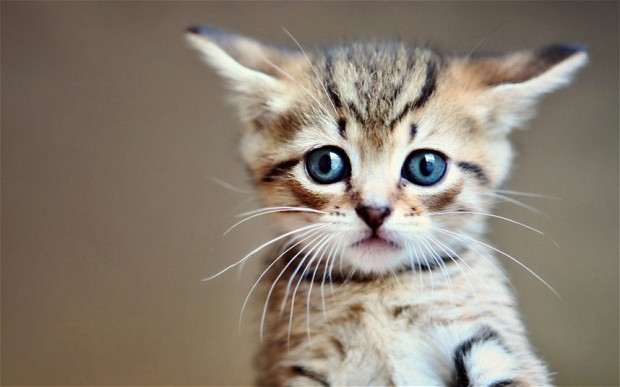
\includegraphics[height=250px, width=350px]{cat1.jpg}
\caption{First picture, this is a kitten, not a use case diagram}
\label{cat1}
\end{figure}

\subsection{Interface Mockups}
At first, this will largely be completely made up, as you get further along in your project, and closer to a final product, this will typically become simple screenshots of your running application.

In this subsection, you will be showing what the screen should look like as the user moves through various use cases (make sure to tie the interface mockups back to the specific use cases they illustrate).



\section{Project Timeline}
Go back to your notes and look up a typical project development life cycle for the Waterfall approach.  How will you follow this life cycle over the remainder of this semester?  This will usually involve a chart showing your proposed timeline, with specific milestones plotted out.  Make sure you have deliverable dates from the course schedule listed, with a plan to meet them (NOTE: these are generally optimistic deadlines).

\section{Project Structure}
At first, this will be a little empty (it will need to be filled in by the time you turn in your final report).  This is your chance to discuss all of your design decisions (consider this the README's big brother).

\subsection{UML Outline}
Show the full structure of your program.  Make sure to keep on updating this section as your project evolves (you often start out with one plan, but end up modifying things as you move along).  As a note, while Dia fails miserably at generating pdfs (probably my fault), I have had much success with png files.  Make sure to wrap your images in a \texttt{figure} environment, and to reference with the \texttt{ref} command.  For example, see Figure \ref{cat2}.

\begin{figure}[ht!]
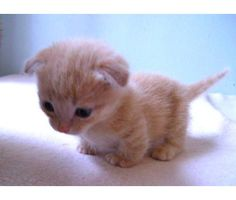
\includegraphics[scale=1.5]{cat2.jpg}
\caption{Your figures should be in the \emph{figure} environment, and have captions.  Should also be of diagrams pertaining to your project, not random internet kittens}
\label{cat2}
\end{figure}


\subsection{Design Patterns Used}
Make sure to actually use at least 2 design patterns from this class.  This is not normally part of such documentation, but largely just specific to this class -- I want to see you use the patterns!


\section{Results}
This section will start out a little vague, but it should grow as your project evolves.  With each deliverable you hand in, give me a final summary of where your project stands.  By the end, this should be a reflective section discussing how many of your original goals you managed to attain/how many desired use cases you implemented/how many extra features you added.

\subsection{Future Work}
Where are you going next with your project?
For early deliverables, what are your next steps?  (HINT: you will typically want to look back at your timeline and evaluate: did you meet your expected goals?  Are you ahead of schedule?  Did you decide to shift gears and implement a new feature?)
By the end, what do you plan on doing with this project?  Will you try to sell it?  Set it on fire?  Link to it on your resume and forget it exists?




\begin{thebibliography}{1}

\bibitem{IEEEhowto:kopka}
H.~Kopka and P.~W. Daly, \emph{A Guide to \LaTeX}, 3rd~ed.\hskip 1em plus
  0.5em minus 0.4em\relax Harlow, England: Addison-Wesley, 1999.

\end{thebibliography}



\begin{IEEEbiography}{Michael Shell}
Biography text here.
\end{IEEEbiography}

% if you will not have a photo at all:
\begin{IEEEbiographynophoto}{John Doe}
Biography text here.
\end{IEEEbiographynophoto}

% insert where needed to balance the two columns on the last page with
% biographies
%\newpage

\begin{IEEEbiographynophoto}{Jane Doe}
Biography text here.
\end{IEEEbiographynophoto}





% that's all folks
\end{document}


